%%%%%%%%%%%%%%
%% Run LaTeX on this file several times to get Table of Contents,
%% cross-references, and citations.

%% If you have font problems, you may edit the w-bookps.sty file
%% to customize the font names to match those on your system.

%% w-bksamp.tex. Current Version: Feb 16, 2012
%%%%%%%%%%%%%%%%%%%%%%%%%%%%%%%%%%%%%%%%%%%%%%%%%%%%%%%%%%%%%%%%
%
%  Sample file for
%  Wiley Book Style, Design No.: SD 001B, 7x10
%  Wiley Book Style, Design No.: SD 004B, 6x9
%
%
%  Prepared by Amy Hendrickson, TeXnology Inc.
%  http://www.texnology.com
%%%%%%%%%%%%%%%%%%%%%%%%%%%%%%%%%%%%%%%%%%%%%%%%%%%%%%%%%%%%%%%%

%%%%%%%%%%%%%
% 7x10
%\documentclass{wileySev}

% 6x9
\documentclass{wileySix}

\usepackage{graphicx}
\usepackage{listings}
\usepackage{float}
\usepackage{indentfirst}

\usepackage{color}
 
\definecolor{codegreen}{rgb}{0,0.6,0}
\definecolor{codegray}{rgb}{0.5,0.5,0.5}
\definecolor{codepurple}{rgb}{0.58,0,0.82}
\definecolor{backcolour}{rgb}{0.95,0.95,0.92}
 
\lstdefinestyle{mystyle}{
    backgroundcolor=\color{backcolour},   
    commentstyle=\color{codegreen},
    keywordstyle=\color{magenta},
    numberstyle=\tiny\color{codegray},
    stringstyle=\color{codepurple},
    basicstyle=\footnotesize,
    breakatwhitespace=false,         
    breaklines=true,                 
    captionpos=b,                    
    keepspaces=true,                 
    numbers=left,                    
    numbersep=5pt,                  
    showspaces=false,                
    showstringspaces=false,
    showtabs=false,                  
    tabsize=2,
    language=sh
}
 
\lstset{style=mystyle}

%%%%%%%
%% for times math: However, this package disables bold math (!)
%% \mathbf{x} will still work, but you will not have bold math
%% in section heads or chapter titles. If you don't use math
%% in those environments, mathptmx might be a good choice.

% \usepackage{mathptmx}

% For PostScript text
\usepackage{w-bookps}

%%%%%%%%%%%%%%%%%%%%%%%%%%%%%%%%%%%%%%%%%%%%%%%%%%%%%%%%%%%%%%%%
%% Other packages you might want to use:

% for chapter bibliography made with BibTeX
% \usepackage{chapterbib}

% for multiple indices
% \usepackage{multind}

% for answers to problems
% \usepackage{answers}

%%%%%%%%%%%%%%%%%%%%%%%%%%%%%%
%% Change options here if you want:
%%
%% How many levels of section head would you like numbered?
%% 0= no section numbers, 1= section, 2= subsection, 3= subsubsection
%%==>>
\setcounter{secnumdepth}{3}

%% How many levels of section head would you like to appear in the
%% Table of Contents?
%% 0= chapter titles, 1= section titles, 2= subsection titles, 
%% 3= subsubsection titles.
%%==>>
\setcounter{tocdepth}{2}

%% Cropmarks? good for final page makeup
%% \docropmarks

%%%%%%%%%%%%%%%%%%%%%%%%%%%%%%
%
% DRAFT
%
% Uncomment to get double spacing between lines, current date and time
% printed at bottom of page.
% \draft
% (If you want to keep tables from becoming double spaced also uncomment
% this):
% \renewcommand{\arraystretch}{0.6}
%%%%%%%%%%%%%%%%%%%%%%%%%%%%%%

%%%%%%% Demo of section head containing sample macro:
%% To get a macro to expand correctly in a section head, with upper and
%% lower case math, put the definition and set the box 
%% before \begin{document}, so that when it appears in the 
%% table of contents it will also work:

\newcommand{\VT}[1]{\ensuremath{{V_{T#1}}}}

%% use a box to expand the macro before we put it into the section head:

\newbox\sectsavebox
\setbox\sectsavebox=\hbox{\boldmath\VT{xyz}}

%%%%%%%%%%%%%%%%% End Demo


\begin{document}


\booktitle{APLIKASI QEUANGANS}
\subtitle{Dengan Android}

\authors{Faris Muhammad Ihsan, Syabriena Putri Veriane\\
\affil{Politeknik Pos Indonesia}
%Floyd J. Fowler, Jr.\\
%\affil{University of New Mexico}
}

\offprintinfo{Cerdas Menguasai Git, First Edition}{Rolly M. Awangga}

%% Can use \\ if title, and edition are too wide, ie,
%% \offprintinfo{Survey Methodology,\\ Second Edition}{Robert M. Groves}

%%%%%%%%%%%%%%%%%%%%%%%%%%%%%%
%% 
\halftitlepage

\titlepage


\begin{copyrightpage}{2019}
%Survey Methodology / Robert M. Groves . . . [et al.].
%\       p. cm.---(Wiley series in survey methodology)
%\    ``Wiley-Interscience."
%\    Includes bibliographical references and index.
%\    ISBN 0-471-48348-6 (pbk.)
%\    1. Surveys---Methodology.  2. Social 
%\  sciences---Research---Statistical methods.  I. Groves, Robert M.  II. %
%Series.\\
%
%HA31.2.S873 2007
%001.4'33---dc22                                             2004044064
\end{copyrightpage}

\dedication{`Jika Kamu tidak dapat menahan lelahnya belajar, 
Maka kamu harus sanggup menahan perihnya Kebodohan.'
~Imam Syafi'i~}

\begin{contributors}
\name{Rolly Maulana Awangga,} Informatics Research Center., Politeknik Pos Indonesia, Bandung,
Indonesia



\end{contributors}

\contentsinbrief
\tableofcontents
\listoffigures
\listoftables
\lstlistoflistings


\begin{foreword}
Sepatah kata dari Kaprodi, Kabag Kemahasiswaan dan Mahasiswa
\end{foreword}

\begin{preface}
Buku ini diciptakan bagi yang awam dengan git sekalipun.

\prefaceauthor{R. M. Awangga}
\where{Bandung, Jawa Barat\\
Februari, 2019}
\end{preface}


\begin{acknowledgments}
Terima kasih atas semua masukan dari para mahasiswa agar bisa membuat buku ini 
lebih baik dan lebih mudah dimengerti.

Terima kasih ini juga ditujukan khusus untuk team IRC yang 
telah fokus untuk belajar dan memahami bagaimana buku ini mendampingi proses 
Intership.
\authorinitials{R. M. A.}
\end{acknowledgments}

\begin{acronyms}
\acro{ACGIH}{American Conference of Governmental Industrial Hygienists}
\acro{AEC}{Atomic Energy Commission}
\acro{OSHA}{Occupational Health and Safety Commission}
\acro{SAMA}{Scientific Apparatus Makers Association}
\end{acronyms}

\begin{glossary}
\term{git}Merupakan manajemen sumber kode yang dibuat oleh linus torvald.

\term{bash}Merupakan bahasa sistem operasi berbasiskan *NIX.

\term{linux}Sistem operasi berbasis sumber kode terbuka yang dibuat oleh Linus Torvald
\end{glossary}

\begin{symbols}
\term{A}Amplitude

\term{\hbox{\&}}Propositional logic symbol 

\term{a}Filter Coefficient

\bigskip

\term{\mathcal{B}}Number of Beats
\end{symbols}

\begin{introduction}

%% optional, but if you want to list author:

\introauthor{Rolly Maulana Awangga, S.T., M.T.}
{Informatics Research Center\\
Bandung, Jawa Barat, Indonesia}

Pada era disruptif  \index{disruptif}\index{disruptif!modern} 
saat ini. git merupakan sebuah kebutuhan dalam sebuah organisasi pengembangan perangkat lunak.
Buku ini diharapkan bisa menjadi penghantar para programmer, analis, IT Operation dan Project Manajer.
Dalam melakukan implementasi git pada diri dan organisasinya.

Rumusnya cuman sebagai contoh aja biar keren\cite{awangga2018sampeu} \cite{maulani2018analysis}.

\begin{equation}
ABC {\cal DEF} \alpha\beta\Gamma\Delta\sum^{abc}_{def}
\end{equation}

\end{introduction}

%%%%%%%%%%%%%%%%%%Isi Buku_
\chapter{Sejarah Android}
\section{Sejarah Android}

\begin{figure}[H]
    \centering
    
\includegraphics[scale=0.2]{pictures/logo_android.jpg}
    \caption{Logo Android}
\end{figure}

Android adalah sistem operasi dengan basis linux yang dirancang untuk perangkat yang bergerak atau layar sentuh \textit{touchscreen} seperti telepon pintar \textit{smartphone} dan \textit{tablet}. Android merupakan sistem operasi \textit{open source} (aplikasi yang tidak dipegang hanya untuk seorang saja tetapi orang lain bisa menggunakan \textit{sourcecode} tersebut). Android ini mengunakan lisensi dari Google yang kodenya tersebut berada dibawah Lisensi \textit{Apache}. Lisensi \textit{Apache} merupakan lisensi yang bebas untuk \textit{software} yang ditulis oleh \textit{Apache Software Foundation} (ASF).

Android berdiri pada bulan Oktober 1980, tepatnya di Palo Alto,  California. Android ini didirikan oleh Andy Rubin, Rich Muner, Nick Sears, dan Chris White. Android dikembangkan oleh perusahaan dengan nama \textit{Ancroid.inc}. Pada tahun 2005 perusahaan tersebut mendapatkan dukungan finansial dari \textit{google.inc}

Pada awalnya Android tidak dibbuat untuk ponsel, namun android pertama kali dibuat untuk kamera digital. Tetapi, dengan melihat peluang yang lebih besar jika Android digunakan untuk perangkat \textit{mobile}, maka Android digunakan pada perangkat \textit{mobile} yang ditujukan untuk menyaingi \textit{Symbian} dan \textit{Windows Mobile}.

Secara resmi, Android dirilis pada tahun 2007 bersamaan dengan berdirinya \textit{Open Handset Alliance}. \textit{Open Handset Alliance} merupakan \textit{Open Source Developer} bagi perangkat \textit{mobile} atau seluler. Tahun 2008, \textit{Handphone} pertama yang menggunakan sistem operasi android kemudian dirilis, \textit{handphone} ini bernama \textit{HTC Dream}. Dua tahun setelah perilisan \textit{Handphone} ini, Google menyusul dengan merilis \textit{Smartphone} dengan seri \textit{Nexus One} yang proses pembuatannya dibantu oleh \textit{HTC}. Dengan dirilisnya \textit{Handphone} tersebut, memancing kemunculan-kemunculan berbagai brand dari \textit{OEM} yang bermacam-macam. Dimulai dari \textit{Samsung, Lenovo, HTC, ASUS, LG} dan masih banyak lagi.

\begin{figure}[!htbp]
    \centering
    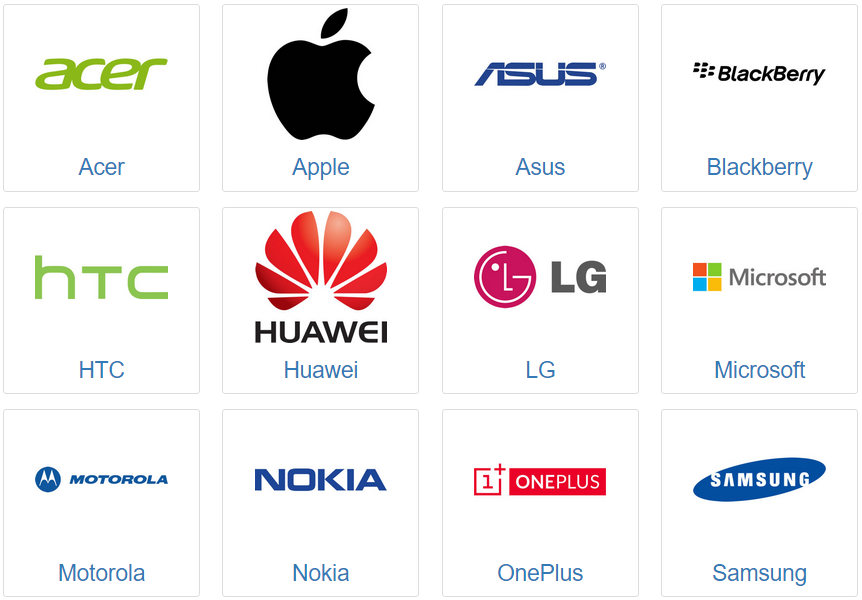
\includegraphics[scale = 0.3]{pictures/merk-OEM-Android.png}
    \caption{OEM Android Smartphone}
\end{figure}

Selain berfokus pada \textit{smartphone}, Google juga banyak mengembangkan aplikasi Android untuk perangkay lainnya. Contohnya Google mengembangkan Android TV yang digunakan untuk televisi, Android Auto yang digunakan pada, dan Android Wear pada jam tangan. Aplikasi android tersebut memiliki \textit{Interface} yang berbeda beda sesuai dengan kebutuhan dan fungsionalitasnya masing-masing. 

\textit{Open Source Code} dan lisensi yang diguakan pada Android tentunya dapat membuat Sistem Operasi ini dapat diubah-ubah dan dimodifikasi dengan bebas yang kemudian dapat di distribusikan oleh para \textit{developer} Android itu sendiri. Selain mudah untuk digunakan, Android memiliki \textit{Developer Community} (Komunitas Pengembang) sendiri yang dapat memperluas fungsionalitas dari perangkat yang umumnya digunakan menggunakan bahasa pemrograman \textit{Java}. Selain \textit{java}, Android ini juga dapat menggunakan bahasa pemrograman \textit{Kotlin}. Lebih dari Satu juta aplikasi kemudian tersedia untuk android, dan miliaran aplikasi telah melakukan di\textit{download} dari \textit{Google Play} (toko utama yang berisi aplikasi-aplikasi dari Android)

Dimulai sejak tahun 2008, Android melakukan pembaruan untuk meningkatkan kinerja aplikasinya secara bertahap dengan cara menambahkan fitur-fitur yang baru dan memperbaiki \textit{error} dan \textit{bug} yang terdapat pada produk dengan versi yang sebelumnya. Setiap versi dari android biasanya disusun dengan nama alfabetis dan nama yang digunakan adalah nama makanan-makanan yang ringan atau cemilan. Sebagai contoh pada android versi 7.0 yang diberi nama Android \textit{Nougat}, Kemudian Android 8.0 yang diberi nama \textit{Oreo} dan seterusnya. 

\section{Versi Pada Android}
Pada awal kemunculan Android, Android telah mengeluarkan banyak versi. Setiap versi dari android ini tentunya memiliki fitur-fiturnya masing-masing sesuai dengan perkembangan zaman. Hal ini tentunya sebagai cara agar mengalahkan pesaingnya yang menggunakan OS yang lainnya seperti Apple iOS, Windows, Blackberry, Symbian dan lainnya. 
\begin{enumerate}

\item Android 1.0 \textbf{Apple Pie}\\
\begin{figure}[!htbp]
    \centering
    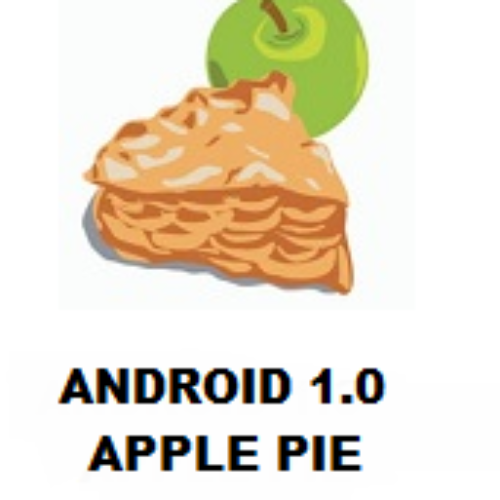
\includegraphics[scale = 0.3]{pictures/asd.jpg}
    \caption{Android Apple Pie}
    \label{}
\end{figure}

Android versi pertama ini merupakan android dengan versi 1.0 yang diberi nama Android \textit{Apple Pie} yang dirilis oleh android  pada 23 September 2008 dan hanya memiliki fitur yang terbatas. Fitur fitur tersebut adalah:

\begin{enumerate}
    \item \textit{Play Store}
    \item Kamera
    \item \textit{Web Browser}
    \item \textit{G-Mail Sychronization}
    \item Kontak
    \item Google Agenda
    \item Google \textit{Maps}
\end{enumerate}
Selain itu, Android versi ini juga sudah mendukung fasilitas youtube. Setidaknya Google dan OHA telas merilis 2 versi saat sebelum Android beta yang dirilis pada bulan November 2007. Pada Android Versi Alpha memiliki sebutan atau \textit{codename} \textit{Astro Boy, Bender,} dan R2-D2.\\

KELEBIHAN
\begin{enumerate}

\item Android Market\\ 
Android market merupakan aplikasi untuk \textit{mendownload} dan \textit{mengupdate} aplikasi yang terinstall melalui toko resmi dari Android.
\item \textit{Web Browser}\\
Android \textit{Web Browser} merupakan aplikasi untuk \textit{searching website}, menampilkan halaman \textit{Web HTML} dan \textit{XHTML} dan dapat digunakan untuk melihat halaman web dengan \textit{fullscreen} dan dapat juga diperbesar.
untuk menampilkan, memperbesar dan melihat dalam layar penuh halaman \textit{Web HTML} dan \textit{XHTML}
\item Kamera
\item Memungkinkan pengelompokan ikon-ikon aplikasi ke dalam satu folder pada bagian layar utama (\textit{homescreen}).
\item Dapat memiliki dan mengakses \textit{E-Mail}, mendukung fasilitas POP3, IMAP4, dan SMTP
\item Sinkronisasi \textit{G-mail} dengan menggunakan aplikasi \textit{G-mail}.
\item Sinkronisasi \textit{Google Contacts} dengan menggunakan aplikasi \textit{People}.
\item Sinkronisasi \textit{Google Calendar} dengan menggunakan aplikasi \textit{Calendar}.
\item Aplikasi \textit{Google Maps} \\
Aplikasi \textit{Google Maps} ini menyediakan informasi mengenai Latitude, derdapat fitur \textit{Street View}, dapat melihat melihat peta dan tampilan melalui citra satelit, menemukan lokasi yang akan dituju dan dapat memberi petunjuk arah saat mengemudi kendaraan maupun saat berjalan-jalan.
\item \textit{Google Sync}\\ 
Fitur ini dapat memungkinkan pengelolaan sinkronisasi pada aplikasi \textit{Gmail, People, dan Calendar}.
\item Google Search\\
Fitur ini dapat memungkinkan pengguna untuk \textit{Searching} sesuatu menggunakan \textit{website}.
\item \textit{Google Talk} \\
\textit{Google Talk} merupakan sebuah aplikasi pesan instan yang diproduksi oleh google
\item Pesan instan, pesan teks (SMS), dan MMS.
\item \textit{Media Player}\\
\textit{Media Player}ini digunakan untuk mengelola, mengimpor, dan memutar file yang mendukung pada berkas penyimpanan. Tetapi, pada versi ini belum menyediakan dukungan \textit{Video} dan \textit{Bluetooth Stereo}
\item Notifikasi\\
Notifikasi ini merupakan fitur yang akan muncul pada status bar, dengan diberikan pilihan pengaturan untuk mengatur \textit{Ringtone}, cahaya \textit{LED} yang dikeluarkan maupun nada getar.
\item \textit{Voice Dialer}\\ 
\textit{Voice Dialer} ini memberikan akses kepada pengguna untuk memanggil kontak tanpa harus mengetikan nama ataupun nomor telepon orang yang akan dituju.
\item Wallpaper\\ 
Fitur ini dapat digunakan pengguna untuk mengatur gambar \textit{Wallpaper} pada \textit{Homescreen} perangkat android pengguna. 
\item \textit{Youtube Video Player}
\item Fitur Pendukung Lainnya seperti:
\begin{enumerate}
    \item Jam Alarm
    \item Kalkulator
    \item Panggilan
    \item \textit{Homescreen Launcher}
    \item Galeri
    \item Pengaturan
\end{enumerate}
\item Wi-Fi
\item Bluetooth
\end{enumerate}

KEKURANGAN
\begin{enumerate}
    \item Versi Android ini pada awalnya belum memiliki nama yang cocok sehingga tidak diberi nama dan hal tersebut dapat membuat bingung masyarakat karena tidak akan mudah untuk diingat.
\end{enumerate}


\item Android 1.1 \textbf{Banana Bread}\\
\begin{figure}[!htbp]
    \centering
    
\includegraphics[scale = 1.2]{pictures/android-banana-bread.jpg}
    \caption{Android Banana Bread}
    \label{}
\end{figure}

Sistem Operasi android yang rilis selanjutnya yaitu Banana Bread, rilis pada bulan Februari 2009. Dan fiturnya yaitu tidak jauh berbeda dengan versi sebelumnya. HTC merupakan salah satu smartphone Android pertama yang menggunakan versi ini. Android 1.1 juga dikenal dengan “Petit Four“, meskipun nama ini tidak digunakan secara resmi. Versi ini memperbaiki beberapa bug, mengubah API Android, dan menambahkan beberapa fitur:
\begin{enumerate}
    \item Rincian dan tinjauan tersedia saat pengguna mencari lokasi bisnis pada Peta.
    \item Kemampuan untuk menampilkan/meenyembunyikan tombol panggilan.
    \item Kemampuan untuk menyimpan lampiran pada pesan.
    \item Menambah dukungan marquee pada tata ruang sistem.
\end{enumerate}


\item Android 1.5 \textbf{Cupcake}\\
\begin{figure}[!htbp]
    \centering
    
\includegraphics[scale = 0.3]{pictures/android-cupcake.jpg}
    \caption{Android Cupcake}
    \label{}
\end{figure}

Dirilis pada awal bulan April 2009 dan juga tidak berbeda dengan versi Android sebelumnya. Hanya saja terdapat fitur tambahan seperti sudah Support Bluetooth A2DP, AVRCP, Soft-keyboard dengan prediksi text dan record atau watch videos. ersi ini adalah rilis pertama yang secara resmi menggunakan nama kode berdasarkan nama-nama makanan pencuci mulut (“Cupcake”), nama yang kemudian digunakan untuk semua versi rilis selanjutnya. Pembaruan pada versi ini termasuk beberapa fitur baru dan perubahan UI:
\begin{enumerate}
    \item Dukungan papan ketik virtual pihak ketiga dengan prediksi teks dan kamus pengguna
    \item Dukungan Widget – tampilan aplikasi miniatur yang tertanam dalam aplikasi lain dan menerima pembaruan secara periodik
    \item Kemampuan merekam dan memutar video berformat MPEG-4 dan 3GP
    \item Kemampuan memasangkan (pairing) dan dukungan stereo bagi Bluetooth (A2DP dan AVRCP)
    \item Fitur salin dan tempel pada penjelajah web
    \item Foto pengguna ditampilkan pada kontak favorit
    \item Tanggal/waktu ditampilkan pada log panggilan, dan akses satu sentuhan ke nomor kontak dari log panggilan
    \item Transisi layar animasi
    \item Opsi memutar-otomatis
    \item Animasi boot baru
    \item Kemampuan untuk mengunggah video ke YouTube
    \item Kemampuan untuk mengunggah foto ke Picasa
\end{enumerate}


\item Android 1.6 \textbf{Donut}\\
\begin{figure}[!htbp]
    \centering
    
\includegraphics[scale=0.5]{pictures/android_donut.jpg}
    \caption{Android Donut}
    \label{}
\end{figure}

Android Donut dirilis pada 15 September 2009, dan terdapat fitur tambahan seperti Gesture Framework hingga Turn-by-turn navigation. Kemudian, Android ini juga terlihat lebih sempurna pada saat itu. Dengan minimnya bug, ditambah lebih lengkapnya berbagai fitur yang disediakan oleh Google. Fitur-fitur barunya adalah sebagai berikut:
\begin{enumerate}
    \item Entri pencarian teks dan suara diperluas, termasuk menyertakan riwayat bookmark, kontak, dan web
    \item Kemampuan bagi para pengembang untuk menyertakan konten mereka pada hasil pencarian
    \item Mesin sintesis pengucapan multibahasa yang memungkinkan aplikasi Android tertentu mampu mengucapkan teks
    \item Pencarian yang lebih mudah dan kemampuan untuk melihat cuplikan aplikasi di Android Market
    \item Galeri, kamera, dan perekam video yang lebih terintegrasi, dengan akses kamera yang lebih cepat
    \item Kemampuan memilih banyak foto untuk dihapus
    Pembaruan dukungan teknologi bagi CDMA/EVDO, 802.1x, VPN, dan mesin pengucap teks
    \item Dukungan bagi resolusi layar WVGA
    \item Peningkatan kecepatan dalam pencarian dan aplikasi kamera
    \item Perluasan kerangka kerja Gestur dan penambahan perkakas pengembangan GestureBuilder.
\end{enumerate}

KEKURANGAN\\
\begin{enumerate}
    \item Tidak semua aplikasi (.apk) bisa di install di sini.
    \item Music playernya belum ada equalizernya.
    \item Android market yang tidak integrated
    \item Keypad nya lemot dan touch responsiveness nya kurang sip daripada versi sesudahnya
\end{enumerate}


\item Android 2.0 \textbf{Eclair} (API level 5)\\
\begin{figure}[!htbp]
    \centering
    
\includegraphics[scale=0.3]{pictures/android-eclair.jpg}
    \caption{Logo Android Eclair}
    \label{}
\end{figure}

Android versi 2.0 ini bernama Eclair dan dirilis pada 26 Oktober 2009 silam. Selain terdapat bluetooth, versi ini juga mendapatkan fitur tambahan seperti multi-touch, Live Wallpaper dan juga flash kamera. Kemudian, beberapa fitur yang dapat anda nikmati dalam versi eclair adalah HTML, Digital zoom, Support Microsoft Exchange, dan Updated UI. Perubahan pada versi ini meliputi:
\begin{enumerate}
    \item Sinkronisasi akun diperluas, yang memungkinkan pengguna menambahkan beberapa akun untuk sinkronisasi surel dan kontak
    \item Dukungan surel Microsoft Exchange, dengan kemampuan menjelajah surel dari beberapa akun dalam satu halaman
    \item Dukungan Bluetooth 2.1
    \item Kemampuan untuk memilih foto kontak dan opsi untuk memanggil, mengirim SMS atau surel kepada kontak yang bersangkutan
    \item Kemampuan untuk mencari semua SMS dan MMS tersimpan, pesan terlama akan dihapus jika batas yang ditentukan sudah tercapai.
    \item Menambahkan sejumlah fitur pada kamera, termasuk dukungan kilat (flash), perbesaran digital, mode skin, kejernihan, efek warna, dan fokus makro.
    \item Peningkatan kecepatan mengetik pada papan ketik virtual, dengan dukungan kamus yang mempelajari penggunaan kata-kata, termasuk nama kontak sebagai saran
    \item UI penjelajah web yang baru, dengan fitur bookmark thumbnail, double-tap zoom, dan dukungan bagi HTML5
    \item Penyempurnaan tampilan agenda kalender; menampilkan status menghadiri untuk setiap undangan, dan kemampuan untuk mengundang tamu baru ke acara tertentu
    \item Mengoptimalkan kecepatan perangkat lunak dan perubahan UI
    \item Dukungan bagi lebih banyak resolusi dan ukuran layar, dengan rasio kecerahan yang lebih baik
    \item Peningkatan Google Maps 3.1.2
    \item MotionEvent ditingkatkan untuk melacak aktivitas multisentuh
    \item Penambahan live wallpaper, yang menampilkan animasi pada latar belakang layar depan
\end{enumerate}

\item Android 2.0.1 \textbf{Eclair} (API level 6)\\
Android versi 2.0 ini bernama Eclair dan dirilis pada 3 Desember 2009. Fitur pada versi ini yaitu :
\begin{enumerate}
    \item Perubahan API minor
    \item Perbaikan bug
    \item perubahan kerangka kerja.
\end{enumerate}

\item Android 2.1 \textbf{Eclair} (API level 7)\\
Android versi 2.0 ini bernama Eclair dan dirilis pada 12 Januari 2010. Fitur pada versi ini yaitu :
\begin{enumerate}
    \item Perubahan kecil pada API 
    \item Perbaikan bug
\end{enumerate}

\item Android 2.2 9 \textbf{Froyo}\\
\begin{figure}[!htbp]
    \centering
    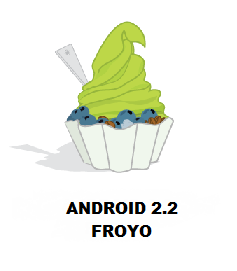
\includegraphics[scale = 0.45]{pictures/android-froyo.png}
    \caption{Android Froyo}
    \label{}
\end{figure}

Pada bulan Mei 2010 lalu, Perusahaan raksasa Google telah merilis Android versi terbaru Yakni adalah Android 2.2 9 (Froyo). Versi ini adalah salah satu sistem operasi Android yang juga telah disempurnakan, tujuannya tentu untuk meningkatkan kecepatan kinerja suatu sistem Android. Dan berikut ini adalah beberapa fitur dan perbaikan yang disediakan oleh Android Froyo :
\begin{enumerate}
    \item Peningkatan Speed
    \item Implementasi JIT
    \item Integrasi mesin JavaScript V8 Chrome pada aplikasi penjelajah web
    \item Dukungan bagi layanan Android Cloud to Device Messaging (C2DM)
    \item Peningkatan dukungan Microsoft Exchange, termasuk kebijakan keamanan, pencarian otomatis, GAL, sinkronisasi kalender, dan pembersihan jarak jauh
    \item Peningkatan peluncur aplikasi dengan jalan pintas ke Telepon dan aplikasi penjelajah web
    \item USB Tethering
    \item Opsi untuk mematikan akses data pada jaringan seluler
    \item Pembaruan aplikasi Market dengan menambahkan fitur pembaruan otomatis
    \item Kontak dan panggilan suara bisa dibagikan melalui Bluetooth
    \item Dukungan bagi Bluetooth-enabled car dan desk docks
    \item Dukungan bagi sejumlah kata sandi alfanumerik
    \item Aplikasi instalasi untuk perluasan memori atau storange
    \item Support file upload pada aplikasi browser
    \item Animated GIFs
    \item Dukungan Adobe Flash
    \item Dukungan tampilan PPI (hingga 320 ppi), misalnya layar 4 inch 720p
    \item Gestur pembesaran pada Galeri
\end{enumerate}

\item Android 2.3 \textbf{Gingerbread}\\
\begin{figure}[!htbp]
    \centering
    
\includegraphics[scale = 0.3]{pictures/android-gingerbread.jpg}
    \caption{Android Gingerbread}
    \label{}
\end{figure}

Pada bulan Desember 2010 lalu, Google merilis kembali Android versi terbarunya yaitu Gingerbread. Yang secara fitur sudah jelas sangat sempurna. Ditambah lagi, Android 2.3 ini juga telah diadopsi oleh salah satu perusahaan Smartphone paling populer, yaitu Samsung dengan menanamkan sistem operasi ini dalam smartphone seri Nexus-nya. Fitur yang disediakan :
\begin{enumerate} 
    \item Memperbarui desain antarmuka pengguna dengan meningkatkan kecepatan dan kesederhanaan
    \item Dukungan bagi resolusi dan ukuran layar ekstra-besar (WXGA dan yang lebih tinggi)
    \item Dukungan bagi telepon internet SIP VoIP
    \item Masukan teks yang lebih cepat dan lebih intuitif pada papan ketik virtual, dengan meningkatkan akurasi, saran teks yang lebih baik, dan modus input suara
    \item Peningkatan fungsi salin/tempel, memungkinkan pengguna untuk memilih kata dengan menekan dan menahan layar
    \item Dukungan bagi Near Field Communication (NFC), memungkinkan pengguna untuk membaca tag NFC yang tertanam dalam poster, stiker, atau iklan
    \item Efek audio baru seperti reverb, equalizer, virtualisasi penyuara kuping, dan bass boost
    \item Download Manager baru, memudahkan pengguna untuk mengakses berkas yang diunduh dari penjelajah web, surel, ataupun dari aplikasi lainnya
    \item Dukungan multi kamera pada perangkat, termasuk kamera depan, jika tersedia
    \item Dukungan bagi pemutar video WebM/VP8, dan audio AAC
    \item Peningkatan manajemen daya dengan peran lebih aktif dalam mengelola aplikasi yang beroperasi terlalu lama
    \item Peningkatan dukungan bagi pengembangan kode asli
    \item Peralihan dari YAFFS ke ext4 pada perangkat yang lebih baru
    \item Peningkatan kualitas audio, grafis, dan masukan bagi pengembang permainan
    \item Dukungan sensor yang lebih banyak (seperti giroskop dan barometer)
\end{enumerate}

\item Android 3.0 - 3.2 6 \textbf{Honeycomb}\\
\begin{figure}[!htbp]
    \centering
    
\includegraphics[scale=0.1]{pictures/android-honeycomb.png}
    \caption{Android Honeycomb}
    \label{}
\end{figure}

Honeycomb adalah salah satu sistem operasi Android versi terbaru yang dirilis pada bulan Februari 2011 silam. Namun, versi ini lebih ditujukkan untuk perangkat Tablet yang mana pada tahun itu sangat laris atau laku dipasaran. Beberapa fitur dan perbaikan pada Android Honeycomb, yaitu :
\begin{enumerate}
    \item Support Multi core
    \item Support Tablet lebih baik
    \item Updated 3D UI
    \item Layar Utama (homescreens) yang dapat diatur
    \item Melihat aplikasi yang barusan dibuka
    \item Menyempurnakan layout keyboard
    \item Transport protocol untuk Media atau Picture video chat Google Talk
    \item Google eBooks
    \item “Private browsing”
    \item System-wide Clipboard
    \item HTTP Live streaming
\end{enumerate}
Update 3.1:
\begin{enumerate}
    \item Peningkatan UI
    \item Open Accessory API
    \item USB host API
    \item Support mouse, joysticks dan gamepad
    \item Widget Home screen yang bisa di atur size atau ukurannya
    \item Notificasi MTP
    \item RTP API untuk audio
\end{enumerate}
Update 3.2:
\begin{enumerate}
    \item Optimise pada berbagai tablets
    \item Mode kompatibilitas display (zoom for fixed sized apps)
    \item Sinkronisasi Media dari SD card
\end{enumerate}
Update 3.2.1:
\begin{enumerate}
    \item Update Android Market merupakan automatic updates yang lebih mudah
    \item Update Google Books
    \item Peningkatan kinerja Wi-Fi
    \item Perbaikan prediksi tulisan tangan dengan huruf Chinese
\end{enumerate}
Update 3.2.2:
\begin{enumerate}
    \item Perbaikan kecil
\end{enumerate}
Update 3.2.4:
\begin{enumerate}
    \item Update tambahan ‘Pay as you go’ bagi tablet
\end{enumerate}
Update 3.2.6
\begin{enumerate}
    \item Perbaikan kecil 
\end{enumerate}

\item Android 4.0 \textbf{Ice Cream Sandwich}\\
\begin{figure}[!htbp]
    \centering
    
\includegraphics[scale = 0.1]{pictures/android-ice-cream-sandwich.png}
    \caption{Android Ice Cream Sandwich}
    \label{}
\end{figure}

Puncak kesempurnaan Android yakni ketika pada versi ini, dimana Ice Cream Sandwich dirilis pada bulan Oktober 2011 silam. Dan operasi sistem ini mulai bekerja dengan baik di semua jenis smartphone apapun. Selain bertambahnya berbagai fitur yang menarik, Ice Cream Sandwich juga merupakan versi yang paling banyak disukai pada saat itu. Bahkan, Android Ice Cream Sandwich juga sudah dilengkapi dengan fitur ekstra multitasking serta notifikasi yang lebih banyak. Pembaruan pada versi ini antara lain:
\begin{enumerate}
    \item Tombol lunak tablet Android 3.x tersedia bagi penggunaan di telepon pintar
    \item Pemisahan widget di tab baru, terletak pada layar yang bersebelahan dengan aplikasi
    \item Pembuatan folder yang lebih mudah, dengan gaya drag-and-drop
    \item Launcher yang bisa dikustomisasi
    \item Peningkatan fitur pesan suara visual, dengan kemampuan untuk mempercepat atau memperlambat kecepatan pesan suara
    \item Fungsi ‘cubit untuk memperbesar’ pada kalender
    \item Pengintegrasian fungsi cuplikan layar (screenshot) dengan menekan dan menahan tombol daya dan volume-turun secara bersamaan
    \item Perbaikan kesalahan koreksi pada papan ketik
    \item Kemampuan untuk mengakses aplikasi secara langsung dari layar kunci (lock screen)
    \item Perbaikan fungsi salin dan tempel
    \item Integrasi suara yang lebih baik dan berkesinambungan
    \item Mode buka kunci identifikasi wajah, fitur yang memungkinkan pengguna untuk membuka perangkat menggunakan perangkat lunak pengenal wajah
    \item Penambahan penjelajah web bawaan Chrome, mampu membuka halaman hingga 16 tab
    \item Sinkronisasi otomatis pada penjelajah web dengan bookmark Chrome pengguna
    \item Penambahan jenis huruf baru, Roboto
    \item Penggunaan data bisa dibatasi, pengguna akan diperingatkan jika penggunaan data sudah mendekati batas tertentu, dan menonaktifkan data yang digunakan ketika batas tersebut terlampaui
    \item Kemampuan untuk mematikan aplikasi yang menggunakan data di latar belakang
    \item Peningkatan fungsi aplikasi kamera dengan fitur-fitur seperti zero shutter lag, time lapse settings, mode panorama, dan kemampuan untuk memperbesar saat merekam video
    \item Penambahan aplikasi pengedit foto bawaan
    \item Tata letak galeri yang baru, bisa dikelola berdasarkan lokasi dan orang
    \item Pemutakhiran aplikasi “People” dengan integrasi pada jejaring sosial
    \item Android Beam, fitur komunikasi area dekat yang memungkinkan dilakukannya pertukaran jarak pendek bookmark web, info kontak, arah, video YouTube, dan data lainnya
    \item Dukungan format gambar WebP
    \item Merekam video 1080p bagi perangkat Android tertentu
    \item Modul kernel Android VPN Framework (AVF) dan TUN (bukan TAP). Sebelum versi 4.0, perangkat lunak VPN membutuhkan rooting.
\end{enumerate}

\item Android 4.1.2 \textbf{Jelly Bean}
\begin{figure}[!htbp]
    \centering
    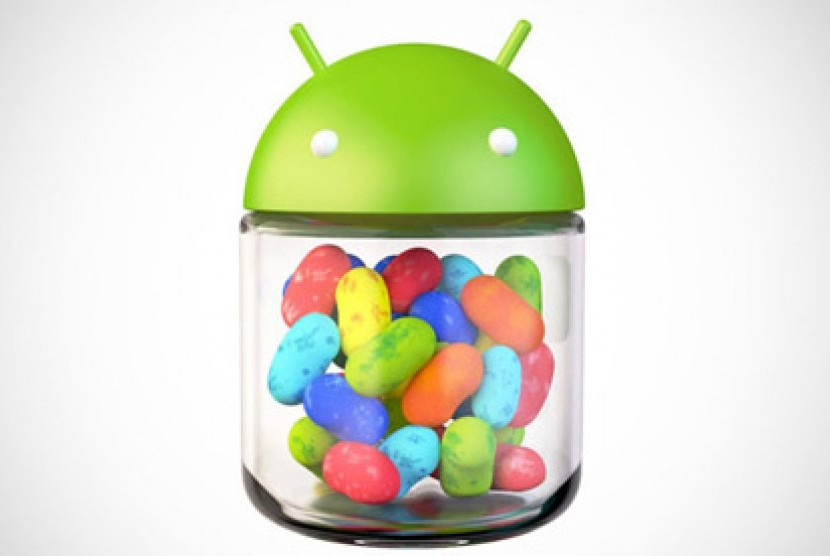
\includegraphics[scale=0.25]{pictures/android-jelly-bean.jpg}
    \caption{Android Jelly Bean}
    \label{}
\end{figure}

Jelly Bean dirilis pada 9 Juli 2012 lewat konferensi I/O Google. Versi ini adalah salah satu versi Android yang kerap mendapatkan update fitur-fitur yang bermanfaat dan menarik, beberapa contohnya semacam memperbaiki rotasi layar, seperti Support resolusi video 4K, Support penulisan huruf Hebrew dan Arabic dari kanan ke kiri, peningkatan kinerja, dan sistem keamanan serta masih banyak lainnya. Fitur yang terdapat pada versi ini adalah : 
\begin{enumerate}
    \item Antarmuka pengguna yang lebih halus:
    \item Waktu vsync pada animasi UI dikelola oleh kerangka kerja Android, termasuk reaksi aplikasi, efek sentuh, komposisi layar, dan penyegaran tampilan
    \item Triple buffering pada grafis
    \item Peningkatan aksesbilitas
    \item Teks dua bahasa dan dukungan bahasa lainnya
    \item Papan ketik yang bisa dimodifikasi oleh pengguna
    \item Perluasan notifikasi
    \item Kemampuan untuk mematikan notifikasi pada aplikasi tertentu
    \item Shortcut dan widget secara otomatis bisa disusun ulang atau diatur ukurannya
    \item Transfer data Bluetooth bagi Android Beam
    \item Diktasi suara luring
    \item Tablet dengan layar kecil bisa menyesuaikan tata letak antarmuka dan layar depan seperti pada telepon pintar
    \item Peningkatan pencarian suara
    \item Peningkatan aplikasi kamera
    \item Google Wallet (pada Nexus 7)
    \item Foto kontak Google+ resolusi tinggi
    \item Aplikasi pencarian Google Now
    \item Audio multi-saluran
    \item Audio USB (bagi suara eksternal DACs)
    \item Audio chaining
    \item Penjelajah web bawaan Android diganti dengan Google Chrome pada perangkat Android pra-instal
    \item Kemampuan untuk menambahkan widget aplikasi tanpa akses root
\end{enumerate}

\item Android 4.4 \textbf{Kitkat}\\
\begin{figure}[!htbp]
    \centering
    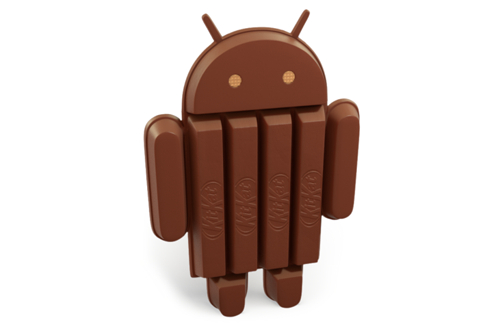
\includegraphics[scale=0.3]{pictures/android-kitkat.jpg}
    \caption{Android Kitkat}
    \label{}
\end{figure}

Android versi inilah yang saat ini banyak dipakai oleh mayoritas masyarakat Indonesia. Kitkat dirilis pada tahun 2013 lalu. pada versi ini, Android banyak mendapatkan pembaharuan/update fitur. Seperti, terdapatnya fitur Screen recording, untuk merekam kegiatan yang terjadi pada layar smartphone, Peningkatan akses notifikasi, New Translucent system UI, System wide settings untuk closed captioning, dan Peningkatan kinerja serta lain sebagainya. Fitur yang terdapat pada versi ini adalah : 
\begin{enumerate}
    \item Pembaruan antarmuka dengan bar status dan navigasi transparan pada layar depan.
    \item Optimasi kinerja pada perangkat dengan spesifikasi yang lebih rendah
    \item Kerangka kerja pencetakan
    \item NFC Host Card Emulation sebagai emulator kartu pintar
    \item WebViews berbasis Chromium
    \item Perluasan fungsionalitas bagi layanan pendengar notifikasi
    \item API umum untuk mengembangkan dan mengelola klien pesan teks, kemampuan untuk menentukan aplikasi SMS standar.
    \item Kerangka kerja baru untuk transisi UI
    \item Kerangka kerja akses penyimpanan untuk mengambil konten dan dokumen dari sumber lain
    \item Sensor batching, Step Detector, dan Counter API
    \item Peningkatan tampilan mode layar penuh, tombol perangkat lunak dan status bar bisa diakses dari tepi dengan cara menggesek
    \item Penyeimbang audio, pemantauan audio, dan peningkatan suara audio
    \item Perekam aktivitas layar yang terintegrasi
    \item Inframerah
    \item Peningkatan aksesibilitas API
    \item Mesin virtual eksperimental baru, ART
    \item Dukungan Bluetooth Message Access Profile (MAP)
\end{enumerate}

\item Android 5.0 \textbf{Lollipop}\\
\begin{figure}[!htbp]
    \centering
    
\includegraphics[scale =0.5]{pictures/android-lolipop.png}
    \caption{Android Lollipop}
    \label{}
\end{figure}

Dirilis pada tahun 2014, Android Lollipop lebih banyak menawarkan fitur tambahan untuk menyempurnakan berbagai fitur yang sudah ada. Dan Nexus 6 merupakan salah satu ponsel yang pertama mencicipi Android Lollipon ini. Selain itu, Google juga lebih menyempurnakan pada kinerja dari Android Lollipop sendiri. Fitur yang terdapat pada versi ini adalah : 
\begin{enumerate}
    \item Desain antarmuka (tampilan) yang dinamakan “Material Design”.
    \item 64-bit ART compiler
    \item Project volta, yang berguna untuk meningkatkan daya hidup baterai 30 persen lebih tahan lama.
    \item ‘factory reset protection’. Fitur ini berguna ketika smartphone hilang, ia tidak bisa direset ulang tanpa memasukkan id google dan kata sandi (password).
\end{enumerate}

\item Android 6.0 \textbf{Marshmallow}\\
\begin{figure}[!htbp]
    \centering
    
\includegraphics[scale=0.3]{pictures/android-marshmallow.jpg}
    \caption{Android Marshmallow}
    \label{}
\end{figure}

Android versi 6.0 dirilis pada tahun 2015 silam, yang banyak membawa pembaharuan. Salah satunya yaitu suda support USB Type-C. Selain itu, Android Marshmallow ini juga terdapat fasilitas autentikasi sidik jari dan daya baterai yang lebih baik. 

Android Marshmallow memperkenalkan model izin yang didesain ulang: sekarang ada hanya delapan kategori izin, dan aplikasi yang tidak lagi secara otomatis diberikan semua hak akses mereka ditentukan pada waktu instalasi. Sebuah sistem opt-in sekarang digunakan, di mana pengguna akan diminta untuk memberikan atau menolak izin individu (seperti kemampuan untuk mengakses kamera atau mikrofon) untuk aplikasi ketika mereka dibutuhkan. Aplikasi mengingat hibah izin mereka, dan mereka dapat disesuaikan oleh pengguna setiap saat. Model izin baru akan digunakan hanya oleh aplikasi yang dikompilasi untuk Marshmallow menggunakan kit pengembangan perangkat lunak (SDK) tersebut, sementara semua aplikasi lainnya akan terus menggunakan model izin sebelumnya.\\

Marshmallow juga memiliki skema manajemen daya baru bernama Doze yang mengurangi tingkat aktivitas aplikasi latar belakang saat perangkat menentukan bahwa itu tidak sedang aktif ditangani oleh pengguna, yang, menurut Google, menggandakan pemakaian baterai perangkat. Hal ini juga memperkenalkan pilihan untuk mengatur ulang semua pengaturan jaringan, tersedia untuk pertama kalinya pada Android, yang membersihkan pengaturan terkait jaringan untuk WI-FI, Bluetooth dan koneksi seluler.

Android Marshmallow memberikan dukungan asli untuk pengenalan sidik jari, memungkinkan penggunaan sidik jari untuk membuka perangkat dan otentikasi Play Store dan pembelian Android Pay; API standar juga tersedia untuk melaksanakan otentikasi berbasis sidik jari dalam aplikasi lain. Android Marshmallow mendukung USB Type-C, termasuk kemampuan untuk menginstruksikan perangkat untuk mengisi daya perangkat lain melalui USB. Marshmallow juga memperkenalkan “pranala yang diverifikasi” yang dapat dikonfigurasi untuk membuka langsung dalam aplikasi tertentu mereka tanpa petunjuk pengguna lanjut.

Versi API Android yang disediakan oleh Marshmallow adalah 23. Alat pengembang Android Marshmallow tersedia di Pengelola SDK di bawah tingkat API “MNC”.

\item Android 7.0 \textbf{Nougat}\\
\begin{figure}[!htbp]
    \centering
    
\includegraphics[scale=0.3]{pictures/android-nougat.jpg}
    \caption{Android Nougat}
    \label{}
\end{figure}

Android Nougat versi 7.0 dirilis pada bulan Agustus 2016 yang lebih meningkatkan pada kinerja versi sebelumnya. Selain itu, Android Nougat juga menambah banyak fitur-fitur baru yang diantaranya seperti sudah dapat multitasking, meningkatkan fitur Doze yang dahulu telah dirilis di versi sebelumnya. Inilah beberapa fitur terbaru yang terdapat pada versi Nougat :
\begin{enumerate}
    \item Support Multi window
    \item Dapat langsung membalas pesan dari menu notifikasi atau jendela.
    \item Tampilan panel notifikasi serta quick settings yang baru.
    \item Mode Doze yang lebih baik, (Doze Mode 2.0)
    \item Menu di antara system settings.
\end{enumerate}

\item Android 8.0 \textbf{Oreo}
\begin{figure}[!htbp]
    \centering
    
\includegraphics[scale=0.3]{pictures/android-oreo.jpg}
    \caption{Android Oreo}
    \label{}
\end{figure}

Android versi Oreo dirilis pada bulan Agustus 2017 lalu. Tentu saja Android Oreo merupakan versi final untuk sekarang ini. Beberapa fiturnya juga turut diluncurkan Google selaku pihak pengelola. Adapun fitur-fiturnya tersebut antara lain yaitu :
\begin{enumerate}
    \item Android O lebih berfokus pada kecepatan dan efisiensi
    \item Kecepatan Boot up 2X lebih cepat
    \item Mode Picture in picture lebih flexibel
    \item Aplikasi yang berjalan di latarbelakang atau background lebih diperketat untuk lebih menghemat battery
    \item Battery lebih tahan lama
    \item Emoji yang diperbaharui dan diperbanyak
\end{enumerate}
\end{enumerate}


\chapter{Android Studio}
\begin{figure}[!htbp]
    \centering
    
\includegraphics[scale=0.1]{pictures/android-studio.png}
    \caption{Android Studio}
    \label{}
\end{figure}
Pertama kali muncul Android Inc merupakan sebuah perusahaan software kecil yang didirikan pada bulan Oktober 2003 di Palo Alto, California, USA. Perusahaan ini dibangun oleh beberapa senior di beberpa perusahaan yang berbasis IT dan Communication, Andy Rubin, Rich Miner, Nick Sears dan Chris White. Rubin menyatakan bahwa, Android Inc Didirikan untuk mewujudkan mobile device yang lebih fleksibel terhadap lokasi dan preferensi pemilik. Sehingga, Android Inc ingin mewujudkan mobile device yang lebih mengerti pemiliknya selain karena OS nya yang open source. Berawal dari konsepan inilah Android Inc ternyata menarik minat Google untuk memilikinya. Maka, pada bulan Agustus 2005, Akhirnya Android Inc diakuisisi oleh Google Inc. dan seluruh sahamnya dibeli oleh Google.

Perusahaan milik Andy Rubin, Rich Miner, Nick Sears dan Chris White tetap di Android Inc yang dibeli Google, sehingga akhirnya mereka pun ikut  menjadi bagian dari raksasa Google dan sejarah Android. Disini mereka mulai menggunakan platform Linux untuk membuat sistem operasi bagi mobile phone.Dari sinilah akhirnya banyak pengembang sistem maupun software yang mengembangkan maupun merancang sistem Android menggunakan software – software yang support dengan Android, Contohnya ialah : Android Studio.

Berikut akan diulas beberapa alasan mengapa memahami Android Studio itu penting untuk dilakukan :
\begin{enumerate}
    \item Dengan mempelajari Android Studio dapat membantu Anda untuk mempercepat pembuatan aplikasi yang Anda inginkan.
    \item Android Studio merupakan sebuah tools yang mudah dipahami dan digunakan.
    \item Dalam satu tools ini Anda bisa mendapatkan berbagai manfaat mulai dari pembuatan aplikasi hingga testing aplikasi.
    \item Belajar Android Studio maka Anda bisa menghemat waktu kerja untuk dapat lebih produktif.
    \item Dapat memperdalam ilmu codingan dengan baik. Karena dalam android studi diberikan beberapa referensi ketika Anda mengetik sintaks. Dengan begitu tentunya Anda akan mencari tahu apa saja kegunaan dari sintaks yang terdapat.
    \item Sarana pembelajaran coding dan pembuatan aplikasi yang baik dan praktis hanya dengan Android Studio.
\end{enumerate}

\section{Android Studio}
Pertama kali Android Studio diumumkan di Google I/O Conference pada tahun 2013 dan dirilis ke publik pada tahun 2014. Sebelum lahirnya Android Studio, aplikasi pada Android dikembangkan dengann Eclipse IDE yaitu IDE Java. Setelah adanya android studio yang open source dapat memudahkan bagi Anda yang ingin membuat aplikasi dengan Android Studio.

Android dapat menyediakan interface untuk Anda dalam membuat aplikasi serta mengelola manajemen filen aplikasi anda.  Untuk bahasa programman anda gunakan adalah Java. Dalam Android Studio, anda hanya tinggal menulis, mengedit, menyimpan  dan testing project beserta dan file lainnya yang ada dalam project itu hanya dengan android studio.

Tidak hanya itu, keunggulan menggunakan Android Studio juga memberi Anda akses ke Android Software Development Kit (SDK). SDK adalah sebuah ekstensi dari kode Java yang memperbolehkannya untuk berjalan dengan mulus di device Android. Untuk, Java nya dibutuhkan untuk menulis program, Android SDK sangat diperlukan untuk menjalankan programnya di Android. Maka dari itu dengan menggabungkan keduanya, Anda memerlukan Android Studio. Sehingga ketika Anda menemukan bug pada aplikasi Anda, Anda bisa mengetahui bug tersebut dengan menggunakan Android Studio untuk memperbaikinya.

Berikut ini adalah beberapa fitur Android Studio:
\begin{enumerate}
    \item Environment yang mempermudah Anda untuk mengembangkan aplikasi untuk Android
    \item Support dalam mengembangkan aplikasi Android TV dan Android Wear
    \item Template untuk menentukan design dan komponen Android
    \item Editor layout dengan interface drag-and-drop
    \item Refactoring dan perbaikan cepat khusus Android
    \item Dukungan build berbasis Gradle
    \item Integrasi ProGuard
    \item Emulator yang cepat dan berbagai fitur didalamnya
    \item Dapat terintegrasi dengan Google Cloud Messaging dan App Engine
    \item Dukungan program basic C++ dan NDK
\end{enumerate}

Android Studio adalah Lingkungan Pengembangan Terpadu (Integrated Development Environment/IDE) resmi untuk pengembangan aplikasi Android, yang didasarkan pada IntelliJ IDEA. Selain sebagai editor kode dan fitur developer IntelliJ yang andal, Android Studio menawarkan banyak fitur yang meningkatkan produktivitas Anda dalam membuat aplikasi Android, seperti:
\begin{enumerate}
    \item Sistem build berbasis Gradle yang fleksibel
    \item Emulator yang cepat dan kaya fitur
    \item Lingkungan terpadu tempat Anda bisa mengembangkan aplikasi untuk semua perangkat Android
    \item Terapkan Perubahan untuk melakukan push pada perubahan kode dan resource ke aplikasi yang sedang berjalan tanpa memulai ulang aplikasi
    \item Template kode dan integrasi GitHub untuk membantu Anda membuat fitur aplikasi umum dan mengimpor kode sampel
    \item Framework dan fitur pengujian yang lengkap
    \item Fitur lint untuk merekam performa, kegunaan, kompatibilitas versi, dan masalah lainnya
    \item Dukungan C++ dan NDK
    \item Dukungan bawaan untuk Google Cloud Platform, yang memudahkan integrasi Google Cloud Messaging dan App Engine
\end{enumerate}

Setiap project di Android Studio berisi satu atau beberapa modul dengan file kode sumber dan file resource. Jenis modul meliputi:
\begin{enumerate} 
   \item Modul aplikasi Android
    \item Modul library
    \item Modul Google App Engine
\end{enumerate}

Secara default, Android Studio menampilkan file project Anda dalam tampilan project Android, seperti yang ditunjukkan. Tampilan ini disusun menurut modul untuk memberikan akses cepat ke file sumber utama project Anda. Semua file build terlihat di tingkat teratas di bagian \textbf{Gradle Script} dan setiap modul aplikasi berisi folder berikut:
\begin{enumerate}
    \item manifests: Berisi file AndroidManifest.xml.
    \item java: Berisi file kode sumber Java, termasuk kode pengujian JUnit.
    \item res: Berisi semua resource non-kode, seperti tata letak XML, string UI, dan gambar bitmap.
\end{enumerate}

Struktur project Android pada disk berbeda dengan representasi tersatukan ini. Untuk melihat struktur file project sebenarnya, pilih \textbf{Project} dari menu drop-down Project.

Anda juga dapat menyesuaikan tampilan file project untuk berfokus pada aspek spesifik dari pengembangan aplikasi Anda. Misalnya, memilih tampilan \textbf{Problems} pada project Anda akan menampilkan link ke file sumber yang berisi error coding dan sintaks yang dikenali, seperti tag penutup elemen XML yang tidak ada dalam file tata letak.

\subsection{Langkah Download Android Studio}
Cara mendownload Android studio cukup mudah yaitu dengan \textbf{https://developer.android.com/studio/?gclid=Cj0KEQiAm-CyBRDx65nBhcmVtbIBEiQA7zm8lWCaBd9n9KYYunFXxXsQCPojBVHk5eIH4p9CWM1eLfUaAmd28P8HAQ} yang merupakan laman website resmi Android dan terdapat SDK berbagai macam jenis didalamnya. Tetapi untuk menjalankan Android Studio Anda juga perlu mendownload Java Development Kit dengan \textbf{https://www.oracle.com/technetwork/java/javase/downloads/jdk8-downloads-2133151.html}.

Berikut ini adalah syarat instalasi untuk berbagai sistem operasi :
Windows OS
\begin{enumerate}
    \item Microsoft Windows 7/8/10
    \item Minimum RAM 2GB, direkomendasikan Anda menggunakan RAM 8GB
    \item Minimum space disk tersedia 2GB, tetapi Anda direkomendasikan menyediakan 4GB (500MB untuk IDE, 1,5GB untuk Android SDK, dan emulator sistem gambar)
    \item Resolusi minimum 1280  800
    \item Java Development Kit 8
\end{enumerate}

MAC OS
\begin{enumerate}
    \item MAC OS X 10.8.5 atau lebih – sampai dengan 10.11.4 (El Capitan)
    \item Minimum RAM 2GB, direkomendasikan Anda menggunakan RAM 8GB
    \item Minimum space disk tersedia 2GB, tetapi Anda direkomendasikan menyediakan 4GB (500MB untuk IDE, 1,5GB untuk Android SDK, dan emulator sistem gambar)
    \item Resolusi minimum 1280  800
    \item Java Development Kit 6
 \end{enumerate}

LINUX OS
\begin{enumerate}
    \item Desktop GNOME atau KDE
    \item 64-bit distribution yang bisa menjalankan aplikasi 32-bit
    \item GNU C Library (glibc) 2.11 atau versi selanjutnya
    \item Minimum RAM 2GB
    \item Minimum space disk tersedia 2GB, tetapi Anda direkomendasikan menyediakan 4GB
    \item Resolusi minimum 1280  800
    \item Java Development Kit 8
\end{enumerate}


\subsection{Cara Install Android Studio}
Pertama sebelum anda menginstall Android Studio, Anda harus terlebih dahulu menginstal Java Development Kit-nya. Caranya ialah Anda tinggal membuka installer Java Development Kit yang sudah ada mengunduh sebelumnya, kemudian selanjutnya ikuti langkah yang mereka tunjukkan.

Setelah itu, Anda sudah bisa menginstall Android Studio dengan mengikuti langkah di bawah ini:
\begin{enumerate}
\item Buka installer Android Studio yang sudah ada unduh. Kemudian klik Next.
\item Setelah itu, muncul jendela baru yang memberikan Anda beberapa pilihan komponen apa saja yang ingin Anda install beserta versi android nya. Lalu klik Next.
\item Selanjutnya Anda akan melihat License Agreement, pilih I Agree
\item Setelah itu, Anda akan melihat pilihan lokasi penyimpanan file. Anda tidak perlu mengubah directory yang sudah mereka pilih. Anda tinggal klik Default dan file Anda akan disimpan ke directory yang sudah mereka sediakan. Klik Next dan di layar selanjutnya klik Install.
\item Setelah proses instalasinya selesai klik Next. Kalau sudah, Anda akan melihat windows “Completing Android Studio Setup”. Anda tidak perlu mengubah pilihan Start Android Studio dan langsung saja klik Finish.
\item Setelah itu, Anda akan melihat jendela baru dengan 2 pilihan. Checklist pilihan kedua jika kalian belum pernah menginstall IDE Android Studio sebelumnya dan pilih OK.
\item Setelah itu Anda akan melihat layar WELCOME dari Android Studio dan klik Next.
\item Pilih Standard dan klik Next
\item Anda kemudian akan melihat jendela SDK Component Setup. Pilih komponen yang ingin Anda install dan klik Next. Pada layar selanjutnya klik Finish.
\item Anda kemudian akan melihat layar Downloading Component.
\item Setelah unduhan Anda selesai, proses instalasi Android Studio telah selesai. Anda tinggal klik Finish. Kemudian Anda akan melihat jendela Welcome to Android Studio.
\end{enumerate}


%\begin{references}{Ham62}
%\bibitem[Kil76]{kilb}J. S. Kilby,
%``Invention of the Integrated Circuit,'' {\it IEEE Trans. Electron Devices,}
%{\bf ED-23,} 648 (1976).
%
%\bibitem[Ham62]{hamm}R. W. Hamming,
%                 {\it Numerical Methods for Scientists and 
%                 Engineers}, Chapter N-1, McGraw-Hill, 
%                 New York, 1962.
%
%\bibitem[Hu86]{lee}J. Lee, K. Mayaram, and C. Hu, ``A Theoretical
%               Study of Gate/Drain Offset in LDD MOSFETs''
%                     {\it IEEE Electron Device Lett.,} {\bf EDL-7}(3). 152 
%                     (1986).
%
%\bibitem[Ber87]{berm}A. Berenbaum, 
%B. W. Colbry, D.R. Ditzel, R. D Freeman, and 
%K.J. O'Connor, ``A Pipelined 32b Microprocessor with 13 kb of Cache Memory,''
%{it Int. Solid State Circuit Conf., Dig. Tech. Pap.,} p. 34 (1987).
%
%\end{references}


\bibliographystyle{IEEEtran} 
%\def\bibfont{\normalsize}
\bibliography{references}


%%%%%%%%%%%%%%%
%%  The default LaTeX Index
%%  Don't need to add any commands before \begin{document}
\printindex

%%%% Making an index
%% 
%% 1. Make index entries, don't leave any spaces so that they
%% will be sorted correctly.
%% 
%% \index{term}
%% \index{term!subterm}
%% \index{term!subterm!subsubterm}
%% 
%% 2. Run LaTeX several times to produce <filename>.idx
%% 
%% 3. On command line, type  makeindx <filename> which
%% will produce <filename>.ind 
%% 
%% 4. Type \printindex to make the index appear in your book.
%% 
%% 5. If you would like to edit <filename>.ind 
%% you may do so. See docs.pdf for more information.
%% 
%%%%%%%%%%%%%%%%%%%%%%%%%%%%%%

%%%%%%%%%%%%%% Making Multiple Indices %%%%%%%%%%%%%%%%
%% 1. 
%% \usepackage{multind}
%% \makeindex{book}
%% \makeindex{authors}
%% \begin{document}
%% 
%% 2.
%% % add index terms to your book, ie,
%% \index{book}{A term to go to the topic index}
%% \index{authors}{Put this author in the author index}
%% 
%% \index{book}{Cows}
%% \index{book}{Cows!Jersey}
%% \index{book}{Cows!Jersey!Brown}
%% 
%% \index{author}{Douglas Adams}
%% \index{author}{Boethius}
%% \index{author}{Mark Twain}
%% 
%% 3. On command line type 
%% makeindex topic 
%% makeindex authors
%% 
%% 4.
%% this is a Wiley command to make the indices print:
%% \multiprintindex{book}{Topic index}
%% \multiprintindex{authors}{Author index}

\end{document}

